% Proposta A (12/11/2026, pedido do autor): o ARIMA e o GARCH juntos, para a
% seção "Integração entre ARIMA e GARCH" do Cap. I, depois das Figuras 5 (ARIMA)
% e 6 (GARCH). As duas saídas da Figura 5 (sinal da previsão e resíduos) são
% repetidas aqui com as mesmas palavras, para o leitor ligar uma figura à outra.
% Conteúdo só do que o Cap. I já diz (araya2024: resíduos do ARIMA como entrada
% do GARCH; direção pelo sinal da previsão; o GARCH condiciona, impedindo ou
% reduzindo). Mesmo estilo das fig05/fig06. Fora do TG até o autor decidir.
\documentclass[11pt,border=2pt]{standalone}
\usepackage[T1]{fontenc}
\usepackage[utf8]{inputenc}
\usepackage{mathptmx}
\usepackage{tikz}
\usetikzlibrary{arrows.meta,positioning,calc,shapes.geometric}
\tikzset{
  seta/.style={-{Stealth[length=2.2mm]}, semithick},
  caixa/.style={rectangle, draw, semithick, fill=gray!10, rounded corners=2pt,
                align=center, minimum width=50mm, minimum height=10mm, font=\small},
  dado/.style={trapezium, trapezium left angle=75, trapezium right angle=105, draw,
               semithick, fill=white, align=center, minimum height=9mm, font=\small,
               trapezium stretches body},
  pergunta/.style={font=\small\itshape, align=center},
}
\begin{document}
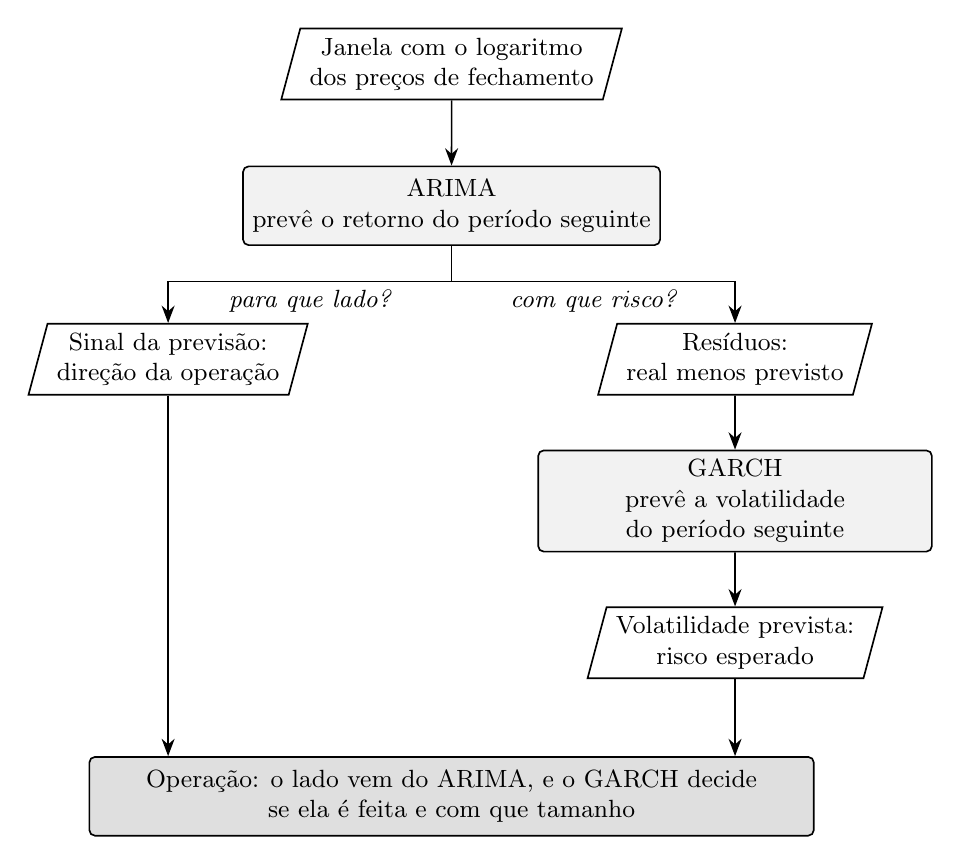
\begin{tikzpicture}
  \node[dado] (ent) at (0,0) {Janela com o logaritmo\\dos preços de fechamento};
  \node[caixa] (arima) at (0,-1.8) {ARIMA\\prevê o retorno do período seguinte};

  \node[dado] (dir) at (-3.6,-3.75) {Sinal da previsão:\\direção da operação};
  \node[dado] (res) at (3.6,-3.75) {Resíduos:\\real menos previsto};
  \node[caixa] (garch) at (3.6,-5.55) {GARCH\\prevê a volatilidade\\do período seguinte};
  \node[dado] (vol) at (3.6,-7.35) {Volatilidade prevista:\\risco esperado};

  \node[caixa, minimum width=92mm, fill=gray!25] (dec) at (0,-9.3)
    {Operação: o lado vem do ARIMA, e o GARCH decide\\se ela é feita e com que tamanho};

  \draw[seta] (ent) -- (arima);
  \draw[seta] (arima.south) -- ++(0,-0.45) -| (dir.north);
  \draw[seta] (arima.south) -- ++(0,-0.45) -| (res.north);
  \draw[seta] (res) -- (garch);
  \draw[seta] (garch) -- (vol);
  \draw[seta] (dir.south) -- (dir.south |- dec.north);
  \draw[seta] (vol.south) -- (vol.south |- dec.north);

  % as duas perguntas que a integração separa (Cap. I, 2º parágrafo da seção)
  \node[pergunta, below] at (-1.8,-2.75) {para que lado?};
  \node[pergunta, below] at (1.8,-2.75) {com que risco?};
\end{tikzpicture}
\end{document}
